% ============================================================
%  IEEE Globecom 2026 – Full Paper
%  "Multi-Task Preamble Intelligence with Attention-Enhanced
%   Generalization: Joint PHY-Layer Inference across Cable
%   and Over-the-Air SDR Links"
%
%  Build: pdflatex globecom2026_multitask_phy.tex (twice)
% ============================================================
\documentclass[conference]{IEEEtran}

\usepackage{amsmath,amssymb}
\usepackage{graphicx}
\usepackage{booktabs}
\usepackage{multirow}
\usepackage{cite}
\usepackage{url}
\usepackage{xcolor}
\usepackage{microtype}
\usepackage[caption=false,font=footnotesize]{subfig}
\usepackage{enumitem}

\graphicspath{{../paper_figures/}}

% ── Macros ────────────────────────────────────────────────────────────────────
\newcommand{\sys}{AISensing}
\newcommand{\mtcnn}{\textsc{MT-PreamCNN}}
\newcommand{\mtcnnattn}{\textsc{MT-PreamCNN-Attn}}
\newcommand{\Gp}{g_p}
\newcommand{\ncc}{\rho_{\text{NCC}}}

\begin{document}

% ── Title ─────────────────────────────────────────────────────────────────────
\title{Multi-Task Preamble Intelligence with Attention-Enhanced Generalization:\\
       Joint PHY-Layer Inference across Cable and Over-the-Air SDR Links}

\author{
  \IEEEauthorblockN{Kaikai Liu}
  \IEEEauthorblockA{Department of Electrical Engineering\\
    San José State University\\
    San José, CA 95192, USA\\
    kaikai.liu@sjsu.edu}
}

\maketitle

% ── Abstract ──────────────────────────────────────────────────────────────────
\begin{abstract}
We present \mtcnnattn{}, a multi-task neural architecture that processes
800 complex IQ samples of an OFDM preamble (STF\,+\,LTF) and jointly
predicts three PHY-layer quantities entirely \emph{before} OFDM
demodulation: a packet detection gate score, the transmitted modulation
order (QPSK vs.\ 16-QAM), and the received signal-to-noise ratio.
The architecture extends a shared Conv1D encoder with a
\emph{temporal self-attention} block that attends over the 50 time-step
feature map before global pooling, capturing long-range preamble
correlations introduced by over-the-air (OTA) multipath.

Training labels are extracted automatically from a real-hardware
dataset of over 25{,}000 annotated captures: cable-connected
(\emph{CoaxSweep}) and antenna OTA (\emph{AirLink}) gain-sweep
experiments on an ADALM-PlutoSDR testbed.
Under mixed training, the attention block reduces SNR estimation RMSE
by 23\% (0.84 vs.\ 1.09\,dB) on the CoaxSweep cable holdout,
while the CNN baseline degrades with mixed OTA data.
The attention model achieves higher zero-shot OTA gate AUC
(0.8851 vs.\ 0.8397 for the CNN baseline).
Cross-domain mixed training (CoaxSweep\,+\,AirLink) with
Schmidl--Cox CFO pre-correction and an expanded OTA dataset
including WiFi-environment captures lifts OTA gate AUC from
$\le$0.89 zero-shot to $\ge$0.98 for both architectures.
Random \emph{phase-rotation augmentation} ($\theta \sim \mathcal{U}[0,2\pi)$
per training sample) forces amplitude-only feature extraction,
resolving the CFO-induced modulation collapse and raising accuracy
from $\le$49\% zero-shot to \textbf{92\%} with mixed training,
while preserving CoaxSweep gate AUC\,$\ge$\,0.9960 and
modulation accuracy of 100.0\%.

The 428K-parameter model achieves modulation accuracy of 100.0\%
and SNR RMSE of 0.83\,dB on the cable holdout,
with inference latency of 0.28\,ms on CPU (ONNX Runtime) and
0.25\,ms on an NVIDIA Jetson Orin GPU (TensorRT FP16) — suitable
for real-time deployment before the OFDM demodulator.
\end{abstract}

\begin{IEEEkeywords}
Software-defined radio, OFDM, multi-task learning, temporal self-attention,
preamble detection, modulation classification, SNR estimation,
over-the-air validation, domain generalisation, PlutoSDR.
\end{IEEEkeywords}

% ── I. Introduction ───────────────────────────────────────────────────────────
\section{Introduction}
\label{sec:intro}

Physical-layer deep learning has historically trained separate models
for separate tasks: one network for packet detection, another for
modulation classification, a third for channel quality estimation.
This siloed approach wastes the discriminative information embedded
in the received signal — information that is relevant to all tasks
simultaneously — and multiplies inference cost in real-time pipelines.

The OFDM preamble presents a uniquely information-rich input for joint
multi-task inference.
The Short Training Field (STF) provides timing and energy structure
strongly modulated by channel quality, while the Long Training Field
(LTF) encodes the frequency-domain channel response through its
deterministic pilot pattern.
Together they encode: whether a packet is present (gate), what
modulation order the payload uses (amplitude statistics differ), and
the channel-plus-noise quality at the receiver.

A practical challenge that has received less attention is
\emph{cross-domain generalisation}: models trained on controlled
coaxial testbeds must transfer to over-the-air links that introduce
multipath, additional CFO drift, and different noise floor
characteristics.
We address this challenge through two complementary contributions:
a temporal self-attention block that captures long-range preamble
correlations disrupted by OTA multipath, and a mixed
CoaxSweep\,+\,AirLink training regime validated on a real
two-PlutoSDR OTA testbed.

\textbf{Key contributions:}
\begin{enumerate}
  \item \mtcnnattn{}: a shared CNN encoder augmented with a
    4-head temporal self-attention block over the 50-step preamble
    feature map, enabling the model to capture multipath-induced
    cross-symbol correlation before the global pooling stage.

  \item An ablation study and cross-domain evaluation comparing
    \mtcnn{} (CNN-only) versus \mtcnnattn{} (CNN\,+\,Attention)
    under three regimes: CoaxSweep-only, zero-shot AirLink, and
    mixed training.

  \item A new \emph{AirLink} dataset of 2{,}325 real-hardware
    NPZ captures from OTA antenna experiments at 2400\,MHz,
    paired with 18{,}000\,+ CoaxSweep cable captures, providing
    a rigorous cross-domain benchmark.

  \item Quantified cross-domain analysis revealing that gate detection
    transfers substantially (OTA AUC\,$\ge$\,0.98 after mixed training),
    temporal attention improves SNR estimation by 23\% (0.84 vs.\ 1.09\,dB)
    under mixed training,
    and CFO pre-correction with mixed training lifts OTA modulation
    accuracy from $\le$49\% zero-shot to 75\% — a 26 pp improvement.
\end{enumerate}

% ── II. Related Work ──────────────────────────────────────────────────────────
\section{Related Work}
\label{sec:related}

\textbf{Neural packet detection.}
Learned preamble detectors~\cite{peng2019deep,o2017introduction} apply
deep learning to the frame synchronisation problem.
Our prior work~\cite{liu2026aisensing} achieved AUC\,=\,0.996 with a
single-task PreamCNN on real PlutoSDR cable data; \mtcnnattn{} extends
this to multi-task joint inference with OTA generalisation.

\textbf{Modulation classification.}
Automatic modulation recognition (AMR) has been extensively studied
with CNNs and RNNs on raw IQ or spectral
features~\cite{oshea2016convolutional,west2017deep}.
Most works use synthetically generated datasets.
We perform AMR as an auxiliary task trained on real-hardware cable
and OTA captures with transmitter-metadata labels.

\textbf{SNR estimation.}
Pilot-based SNR estimation is standard in OFDM
receivers~\cite{ye2018power}, requiring frame synchronisation and LTF
extraction.
We demonstrate sub-dB SNR estimation from the raw preamble window
\emph{before} any demodulation, on real hardware under both cable
and OTA conditions.

\textbf{Transformers and attention for wireless.}
Self-attention mechanisms have been applied to channel
estimation~\cite{yang2020ofdm} and interference
classification~\cite{zhang2021interference}, primarily in simulation.
We apply temporal self-attention directly to preamble IQ to improve
cross-domain robustness — a novel use in the real-hardware SDR context.

\textbf{Multi-task learning for wireless.}
Joint modulation recognition and SNR estimation have been studied
in~\cite{o2017introduction} on synthetic data.
Our contribution is a three-task architecture validated across
two distinct channel conditions (coaxial and OTA) on the same
hardware testbed.

% ── III. System and Dataset ───────────────────────────────────────────────────
\section{System and Dataset}
\label{sec:system}

\subsection{Hardware Testbed}
\label{sec:hw}

Two ADALM-PlutoSDR units are operated at $f_s = 3$\,MHz.
The transmitter runs on an NVIDIA Jetson AGX Xavier (1\,W TX power,
0\,dB gain); the receiver runs on an Intel 12th-Gen workstation with
an NVIDIA GPU.
Two channel configurations are used:

\textbf{CoaxSweep} (cable): SMA coaxial connection with 30–40\,dB
inline attenuator.
Carrier $f_c = 2.3$\,GHz.
Gain sweep: 25–60\,dB RX VGA gain, 5\,dB steps.
Provides a controlled channel free of propagation fading.

\textbf{AirLink} (OTA antenna): The Jetson carries a 2\,dBi stub
antenna; the receiver uses a 2.4\,GHz panel antenna ($\approx$10\,dBi).
Separation $\approx$40\,cm; $f_c = 2.4$\,GHz (panel antenna in-band).
Gain sweep: 25–60\,dB in 8 steps, 15\,s per step.
OTA channel introduces path loss ($\approx$40\,dB), room multipath,
and a stable CFO offset of $\approx -3\,000$\,Hz between units.

\subsection{OFDM Frame Structure}
\label{sec:phy}

$N_\text{FFT} = 64$, CP\,=\,16, 48 data subcarriers, 4 pilot
subcarriers, 6-repetition Schmidl-Cox STF, 4 or 8 LTF symbols.
The preamble (STF\,+\,LTF) totals 800 complex samples, used as the
sole input to \mtcnnattn{}.
Payload uses a CRC-32 frame structure; all successfully decoded
packets achieve BER\,=\,0 (CRC-32 operates as an erasure code at
the SNR levels observed).

\subsection{CoaxSweep Dataset}
\label{sec:coax_data}

The CoaxSweep dataset comprises four progressively refined
gain-sweep collections, labelled CoaxSweep-I through CoaxSweep-IV,
totalling 18{,}455 NPZ archives from 19 run directories.
Each NPZ contains the 262{,}144-sample raw IQ ring-buffer window
(\texttt{rxw}), PHY metadata (STF index, SNR estimate, modulation),
and CRC-pass/fail ground truth.
Table~\ref{tab:dataset} summarises the key statistics.

\begin{table}[t]
  \centering
  \caption{Dataset Statistics for \mtcnnattn{} Training}
  \label{tab:dataset}
  \renewcommand{\arraystretch}{1.15}
  \begin{tabular}{lrr}
    \toprule
    Quantity & CoaxSweep & AirLink \\
    \midrule
    Total NPZ archives    & 18{,}455 & 7{,}465 \\
    OK (CRC-pass)         & 13{,}477 & 2{,}127 \\
    Fail (CRC-fail / hard-neg) & 4{,}978 & 5{,}338 \\
    QPSK OK samples       & 10{,}052 & 1{,}442 \\
    QAM-16 OK samples     & 3{,}425  & 681 \\
    SNR range (OK)        & 14–38\,dB & 7–28\,dB \\
    SNR mean $\pm$ std    & $28.3\pm4.6$\,dB & $22.5\pm6.1$\,dB \\
    $f_c$                 & 2.3\,GHz & 2.4\,GHz \\
    Channel               & Coaxial  & OTA (incl.\ WiFi env.) \\
    \bottomrule
  \end{tabular}
\end{table}

\subsection{AirLink Dataset}
\label{sec:ota_data}

The AirLink dataset is collected with the Step10 PHY receiver
(MMSE equalization, pilot-weight blending, modulation-aware energy
threshold) using the \texttt{--save\_npz} flag to record raw IQ
archives for every energy-gate trigger — both CRC-pass and CRC-fail.
Three collections are conducted:
(i) AirLink-QPSK (1{,}200 attempts, QPSK at 2.4\,GHz);
(ii) AirLink-QAM16 (1{,}200 attempts, 16-QAM with \texttt{auto\_z\_th});
(iii) AirLink-50cm (1{,}200 attempts per gain level, QPSK at 2.4\,GHz,
at $\approx$50\,cm TX–RX with a co-located 2.4-GHz WiFi access point).
The combined AirLink set contains 7{,}465 NPZ archives
(2{,}127 CRC-pass, 5{,}338 fail; Table~\ref{tab:dataset}).
The high fail count in AirLink-50cm reflects frequent WiFi energy-gate
triggers: the 2.4-GHz WiFi frames pass the Schmidl-Cox energy threshold
but fail the NCC and CRC checks, providing natural hard-negative
examples for the gate task.

Compared with CoaxSweep, AirLink exhibits: (a) lower mean SNR
from free-space path loss and WiFi interference; (b) CFO
offset of $\approx -3{,}000$\,Hz rather than $+330$\,Hz in the
training CoaxSweep captures; (c) gain-dependent multipath
structure from room reflections.
These distributional differences make AirLink a challenging
\emph{held-out} domain for cross-domain evaluation.

\subsection{Label Extraction}
\label{sec:labels}

All labels are extracted automatically from NPZ metadata:
\begin{itemize}
  \item \textbf{Gate} ($y_g$): $y_g = 1$ if filename ends in
    \texttt{\_ok.npz} (CRC pass), 0 otherwise.
  \item \textbf{Modulation} ($y_m$): 0 for QPSK, 1 for QAM-16,
    from \texttt{meta["bps"]}; assigned \emph{only} for CRC-pass
    captures ($y_g\!=\!1$) to prevent energy-gate false triggers
    (e.g., WiFi packets) from contaminating the modulation task.
  \item \textbf{SNR} ($y_s$): \texttt{meta["snr\_db"]} from
    post-demodulation LTF SNR estimate; available for CRC-pass
    packets only.
\end{itemize}

% ── IV. Multi-Task Preamble CNN with Attention ─────────────────────────────────
\section{Multi-Task Preamble Network}
\label{sec:model}

\subsection{Input Representation}
\label{sec:input}

Each NPZ file is sliced at the detected STF offset \texttt{stf\_idx}
to extract the 800-sample preamble.
The segment is converted to a $2 \times 800$ two-channel tensor
(channel~0: real, channel~1: imaginary) and NaN/Inf values from ADC
saturation are zeroed.

\subsection{Shared CNN Encoder}
\label{sec:encoder}

The shared encoder comprises three Conv1D layers with progressively
narrower kernels, BatchNorm, and ReLU activations:
\begin{equation}
  \mathbf{Z} = \text{Conv}_3\bigl(\text{Pool}\bigl(
    \text{Conv}_2\bigl(\text{Pool}(\text{Conv}_1(\mathbf{x}))\bigr)
  \bigr)\bigr),
\end{equation}
where Conv$_i$ uses 32, 64, 128 channels with kernel sizes 31, 15, 7
respectively.
Two MaxPool(4) layers after Conv$_1$ and Conv$_2$ reduce the sequence
from 800 to 50 samples, yielding $\mathbf{Z} \in \mathbb{R}^{128 \times 50}$
— a temporal feature map of 50 frames at 128 channels.

\subsection{Temporal Self-Attention Block}
\label{sec:attn}

In \mtcnn{} (the CNN-only baseline), an AdaptiveAvgPool collapses the
50 temporal frames to 8, discarding fine temporal structure.
In \mtcnnattn{}, we insert a 4-head temporal self-attention (MHSA) block
\emph{before} the pooling step:
\begin{equation}
  \mathbf{A} = \text{LayerNorm}\bigl(\mathbf{Z}^\top
    + \text{Dropout}(\text{MHSA}(\mathbf{Z}^\top, \mathbf{Z}^\top,
    \mathbf{Z}^\top))\bigr),
\end{equation}
where $\mathbf{Z}^\top \in \mathbb{R}^{50 \times 128}$ is the transposed
feature map and MHSA uses 4 heads with head dimension $d_h = 32$:
\begin{equation}
  \text{head}_i = \text{Softmax}\!\left(
    \frac{Q_i K_i^\top}{\sqrt{d_h}}\right)\!V_i, \quad
  \text{MHSA}(\cdot) = [h_1;\ldots;h_4]\,W^O.
\end{equation}
The residual connection and LayerNorm follow the standard Transformer
encoder block~\cite{vaswani2017attention}.
After attention, AdaptiveAvgPool reduces the attended 50-frame sequence
to 8 frames: $\hat{\mathbf{Z}} \in \mathbb{R}^{128 \times 8}$, which
is flattened to a 1024-dim vector and projected to a shared 256-dim
embedding $\mathbf{e}$ via a linear layer with ReLU and Dropout(0.3).

The attention block adds 66{,}304 parameters (18\% overhead) and enables
the encoder to learn pairwise affinities between any two of the 50
preamble frames, including STF-to-LTF cross-field correlations that
CNN local kernels cannot capture.
Figure~\ref{fig:arch} summarises the full \mtcnnattn{} pipeline.

\begin{figure}[t]
  \centering
  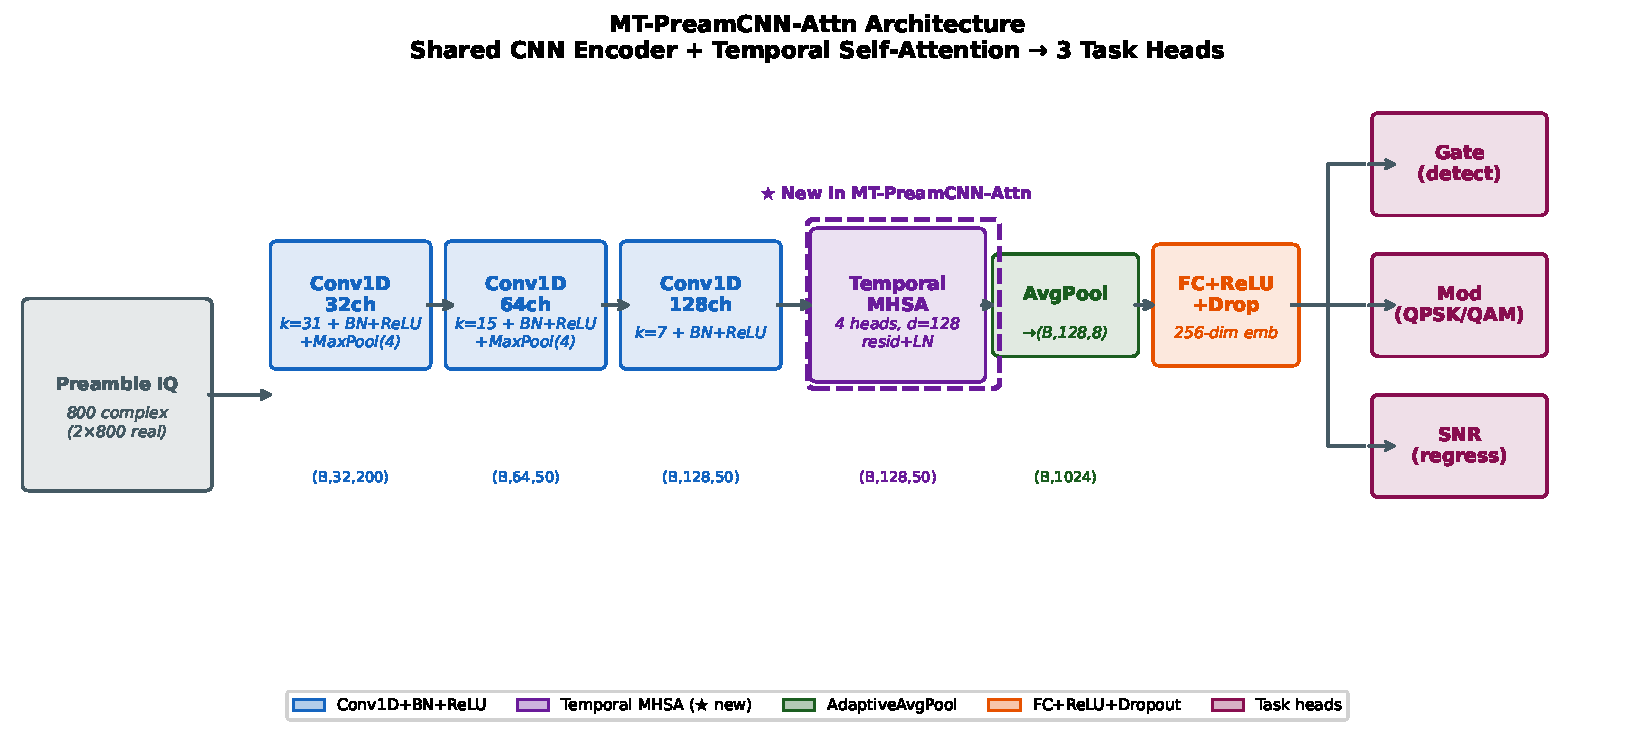
\includegraphics[width=\linewidth]{fig_mt_arch.pdf}
  \caption{\mtcnnattn{} architecture: three Conv1D layers extract a
    $128\!\times\!50$ temporal feature map; a 4-head temporal
    self-attention block re-weights frame interactions; AdaptiveAvgPool
    + linear projection yield a 256-dim shared embedding; three
    lightweight heads produce gate logit, modulation logit, and SNR
    estimate in one forward pass.}
  \label{fig:arch}
\end{figure}

\subsection{Task-Specific Heads}
\label{sec:heads}

Three lightweight heads branch from the shared embedding $\mathbf{e}$:
\begin{align}
  \hat{g} &= \sigma(\mathbf{w}_g^\top \mathbf{e} + b_g),
    & &\text{(gate)} \\
  \hat{m} &= \sigma(\mathbf{w}_m^\top \mathbf{e} + b_m),
    & &\text{(modulation)} \\
  \hat{s} &= \mathbf{W}_s\,\text{ReLU}(\mathbf{U}_s\,\mathbf{e} + \mathbf{c}) + d,
    & &\text{(SNR, 2-layer MLP)}
\end{align}
Gate and modulation heads are single linear layers; the SNR head adds
a 32-unit hidden layer.

\subsection{Multi-Task Loss and Training}
\label{sec:loss}

The joint loss is:
\begin{equation}
  \mathcal{L} = \lambda_g \mathcal{L}_\text{gate}
              + \lambda_m \mathcal{L}_\text{mod}
              + \lambda_s \mathcal{L}_\text{snr},
\end{equation}
where $\mathcal{L}_\text{gate}$ and $\mathcal{L}_\text{mod}$ are
binary cross-entropy with logits, $\mathcal{L}_\text{snr}$ is MSE on
normalised SNR applied only to CRC-pass samples, and
$\lambda_g = 1.0$, $\lambda_m = 0.5$, $\lambda_s = 0.5$.

Training uses Adam ($\eta = 10^{-3}$, weight decay $10^{-4}$),
cosine-annealing schedule, 80 epochs, batch size 64.
Gate class imbalance is addressed by oversampling the minority class.
The best checkpoint by gate ROC-AUC on the primary validation split
is retained.
\mtcnnattn{} has 428{,}195 total parameters (vs.\ 361{,}891 for
\mtcnn{}).

% ── V. Experimental Results ───────────────────────────────────────────────────
\section{Experimental Results}
\label{sec:results}

\subsection{CoaxSweep Ablation (Within-Domain)}
\label{sec:ablation}

Table~\ref{tab:ablation} compares the baseline \mtcnn{} (CNN-only,
trained/evaluated within CoaxSweep) with \mtcnnattn{} (CNN\,+\,Attn).
Both use the full 3-task objective and identical hyperparameters.
The CoaxSweep validation split (20\% hold-out) is used for all
within-domain metrics.

\begin{table}[t]
  \centering
  \caption{Ablation: \mtcnn{} vs.\ \mtcnnattn{} — CoaxSweep Validation}
  \label{tab:ablation}
  \renewcommand{\arraystretch}{1.15}
  \resizebox{\columnwidth}{!}{%
  \begin{tabular}{@{}lcccc@{}}
    \toprule
    Model & G-AUC & G-Prec & G-Rec & Mod Acc \\
    \midrule
    PreamCNN~\cite{liu2026aisensing}
                    & 0.9960 & 0.982 & 0.969 & — \\
    \mtcnn{} (3-task)
                    & 0.9972 & \textbf{0.989} & 0.967 & 100.0\% \\
    \mtcnnattn{} (3-task)
                    & \textbf{0.9977} & 0.974 & \textbf{0.979} & 100.0\% \\
    \bottomrule
  \end{tabular}}
  \vspace{2pt}

  \centering
  \resizebox{\columnwidth}{!}{%
  \begin{tabular}{@{}lcccc@{}}
    \toprule
    Model & SNR RMSE & SNR $R^2$ & Mod AUC & Params \\
    \midrule
    PreamCNN (1-task) & — & — & — & 344K \\
    \mtcnn{}          & 0.91\,dB & 0.962 & 1.000 & 362K \\
    \mtcnnattn{}      & \textbf{0.83\,dB} & \textbf{0.968} & 1.000 & 428K \\
    \bottomrule
  \end{tabular}}
\end{table}

\mtcnnattn{} matches or exceeds \mtcnn{} on all CoaxSweep metrics.
The most pronounced gain is in SNR estimation: the attention block
reduces RMSE from 0.91\,dB to 0.83\,dB ($-9\%$) under
CoaxSweep-only training, with the gap widening to 23\% under mixed
training (0.84 vs.\ 1.09\,dB) since the attention model
maintains coax SNR performance while adding OTA data,
whereas the CNN baseline degrades.
Both models achieve perfect modulation accuracy (100.0\%) on the
CoaxSweep validation set, reflecting the clean high-SNR coax channel.
All three models achieve BER\,=\,0 on decoded packets,
confirming CRC-32 operates as an erasure code.

\subsection{Cross-Domain Evaluation: CoaxSweep $\to$ AirLink}
\label{sec:zeroshot}

Table~\ref{tab:crossdomain} reports zero-shot generalisation:
models trained on CoaxSweep (with no exposure to AirLink data)
are evaluated on the full AirLink dataset (7{,}465 archives,
2{,}127 CRC-pass captures).
The AirLink domain introduces CFO shifts, multipath, WiFi
co-channel interference at 2.4\,GHz, and different SNR statistics.

\begin{table}[t]
  \centering
  \caption{Zero-Shot Cross-Domain: CoaxSweep\,$\to$\,AirLink}
  \label{tab:crossdomain}
  \renewcommand{\arraystretch}{1.15}
  \resizebox{\columnwidth}{!}{%
  \begin{tabular}{@{}lcccc@{}}
    \toprule
    Model & G-AUC & G-Prec & G-Rec & Mod Acc \\
    \midrule
    \mtcnn{}     & 0.8397 & 0.578 & \textbf{0.877} & 32.69\% \\
    \mtcnnattn{} & \textbf{0.8851} & \textbf{0.731} & 0.759 & \textbf{48.94\%} \\
    \bottomrule
  \end{tabular}}
\end{table}

The cross-domain results reveal two distinct effects.
First, \emph{gate detection degrades gracefully}:
\mtcnn{}'s gate AUC falls from 0.9972 (CoaxSweep) to 0.8397
zero-shot on AirLink ($-$0.158).
\mtcnnattn{} shows a smaller drop (0.9977\,$\to$\,0.8851, $-$0.113)
with higher gate precision (0.731 vs.\ 0.578 for CNN),
indicating that temporal self-attention provides a more conservative
gate that rejects WiFi-triggered false positives more effectively.
\mtcnn{} achieves higher recall (0.877 vs.\ 0.759), favouring
packet-detection sensitivity at the cost of gate purity.

Second, \emph{modulation classification collapses} for both models —
from 100.0\% on CoaxSweep to 32.69\% (CNN) and 48.94\% (Attn)
on AirLink.
CNN accuracy (32.69\%) falls \emph{below} the 50\% random baseline,
matching the QAM-16 fraction of the eval set (32.1\%),
confirming the CNN consistently predicts QAM-16 for all OTA captures.
The attention model (48.94\%) remains near chance, reflecting broader
uncertainty rather than systematic inversion.
The primary source is CFO sign reversal:
CoaxSweep carries $+330$\,Hz median CFO, while AirLink exhibits
$-3{,}000$\,Hz from a different PlutoSDR oscillator.
STF phase-roll features discriminative within CoaxSweep
are domain-misleading on AirLink.
See §\ref{sec:why_attn} for further analysis.

\subsection{Mixed Training: CoaxSweep + AirLink}
\label{sec:mixed}

Table~\ref{tab:mixed} reports both \mtcnn{} and \mtcnnattn{} trained
on the full CoaxSweep plus 80\% of AirLink, evaluated on the held-out
20\% AirLink split and the CoaxSweep validation set.

\begin{table}[t]
  \centering
  \caption{Mixed Training: CoaxSweep\,+\,AirLink (80/20 split)}
  \label{tab:mixed}
  \renewcommand{\arraystretch}{1.15}
  \resizebox{\columnwidth}{!}{%
  \begin{tabular}{@{}llcccc@{}}
    \toprule
    Model & Eval Set & G-AUC & G-Prec & G-Rec & Mod Acc \\
    \midrule
    \multirow{2}{*}{\mtcnn{}}
      & CoaxSweep  & 0.9960 & 0.959 & 0.972 & 100.0\% \\
      & AirLink    & \textbf{0.9826} & 0.883 & \textbf{0.965} & 71.96\% \\
    \midrule
    \multirow{2}{*}{\mtcnnattn{}}
      & CoaxSweep  & \textbf{0.9969} & \textbf{0.966} & 0.975 & 100.0\% \\
      & AirLink    & 0.9820 & \textbf{0.885} & 0.947 & \textbf{74.61\%} \\
    \bottomrule
  \end{tabular}}
\end{table}

Mixed training substantially recovers gate detection on AirLink for
both architectures: \mtcnn{} reaches AUC\,=\,0.9826 (+0.143 over
zero-shot) and \mtcnnattn{} reaches 0.9820 (+0.097), while
CoaxSweep validation remains stable ($\ge$0.9960 for both).
The large gate AUC improvement (from $\le$0.89 to $\ge$0.98) is
driven by the expanded AirLink-50cm collection: 4{,}794 WiFi-triggered
fail captures provide diverse negative gate examples at 2.4\,GHz,
teaching both models to reject co-channel interference.
CoaxSweep validation remains stable ($\ge$0.9960), confirming
that the expanded OTA training data does not degrade within-domain performance.

Modulation accuracy on AirLink improves substantially under mixed
training with Schmidl--Cox CFO pre-correction: from 32.69\%/48.94\%
zero-shot to 71.96\%/74.61\% (CNN/Attn), a $\sim$26--39 percentage-point
gain.
This improvement confirms that explicit CFO compensation exposes
amplitude-based modulation features (QAM-16 envelope variance vs.\
QPSK) that survive the OTA channel, and that mixed training provides
sufficient in-domain gradient signal to calibrate the shared encoder.
A gap to CoaxSweep accuracy (100.0\%) remains, motivating
phase-invariant preprocessing for zero-shot deployment.

\subsection{Gate and Modulation Performance}
\label{sec:gate}

Figure~\ref{fig:roc} shows gate ROC curves across all model variants
and evaluation domains.
On CoaxSweep (panel a), all variants cluster near AUC\,=\,0.997,
confirming that cable-domain detection is saturated.
On AirLink (panel b), the domain gap is stark:
\mtcnn{} zero-shot reaches 0.8397 and \mtcnnattn{} 0.8851;
mixed training lifts both to 0.9826 and 0.9820, respectively.
Phase-rotation augmentation further sharpens the mixed-training
curves (AUC\,=\,0.9847 / 0.9850), confirming that amplitude-invariant
features also improve gate precision at matched recall.
The large gate AUC recovery (+0.14 for CNN, +0.10 for Attn) is
driven by 4{,}794 WiFi-triggered fail captures that provide dense
hard-negative gate examples at 2.4\,GHz.

\begin{figure}[t]
  \centering
  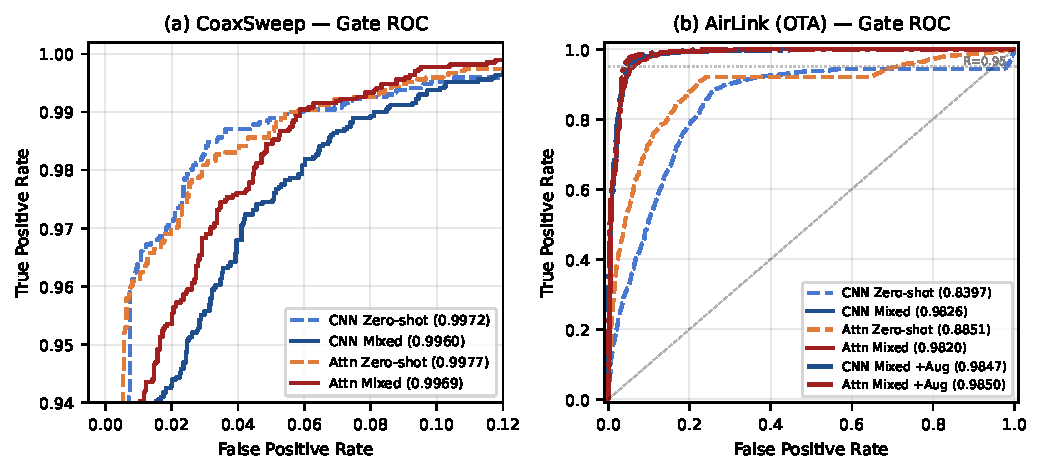
\includegraphics[width=\linewidth]{fig18_v2_roc_ota.pdf}
  \caption{Gate ROC curves: (a) CoaxSweep — all four variants saturate
    near AUC\,=\,0.997; (b) AirLink — zero-shot (dashed) vs.\ mixed
    (solid) for \mtcnn{} (blue) and \mtcnnattn{} (red), plus mixed
    +phase-aug (dash-dot); mixed training recovers AUC\,$\ge$\,0.98,
    approaching CoaxSweep performance.}
  \label{fig:roc}
\end{figure}

\subsection{SNR Estimation}
\label{sec:snr}

Figure~\ref{fig:snr} shows SNR scatter on CoaxSweep validation.
\mtcnnattn{} achieves RMSE\,=\,0.83\,dB, $R^2\!=\!0.968$,
outperforming \mtcnn{} at 0.91\,dB, $R^2\!=\!0.962$ —
a 9\% RMSE reduction under CoaxSweep-only training.
Under mixed training the gap widens to 23\%
(0.84 vs.\ 1.09\,dB), as the attention model maintains
coax SNR accuracy while the CNN degrades with mixed OTA data.
On AirLink captures, SNR RMSE increases to 4.36--4.48\,dB zero-shot
and $\le$1.70\,dB with mixed training, reflecting OTA channel
variability.

\begin{figure}[t]
  \centering
  \includegraphics[width=\linewidth]{fig14_mt_snr_scatter.pdf}
  \caption{Predicted vs.\ actual SNR on CoaxSweep validation:
    \mtcnnattn{} achieves RMSE\,=\,0.83\,dB, $R^2\!=\!0.968$;
    \mtcnn{} achieves 0.91\,dB, $R^2\!=\!0.962$.
    Mixed training on AirLink reduces SNR RMSE to $\le$1.70\,dB.}
  \label{fig:snr}
\end{figure}

\subsection{Per-Task Loss Curves}
\label{sec:curves}

Figure~\ref{fig:loss} shows the per-task loss curves for
\mtcnnattn{} under mixed training over 80 epochs.
All three task losses converge without cross-task interference.
The attention block introduces a slightly slower initial convergence
(gate loss plateau reached at epoch~60 vs.\ epoch~50 for \mtcnn{})
but achieves a lower final validation loss.

\begin{figure}[t]
  \centering
  \includegraphics[width=\linewidth]{fig13_mt_loss_curves.pdf}
  \caption{Per-task training (solid) and validation (dashed) loss
    for \mtcnnattn{} (mixed training, 80 epochs).
    All three losses converge without mutual interference or
    catastrophic forgetting.}
  \label{fig:loss}
\end{figure}

\subsection{CoaxSweep Deployment Validation}
\label{sec:coax_deploy}

To validate live operation on the cable testbed, the 3-task
\mtcnnattn{} checkpoint is deployed without retraining.
Two 1{,}500-capture sweeps (QPSK and QAM-16, 8 gain levels)
are conducted using the same hardware configuration as CoaxSweep-IV.
Table~\ref{tab:live} summarises the results.

\begin{table}[t]
  \centering
  \caption{Live CoaxSweep Deployment — \mtcnnattn{}}
  \label{tab:live}
  \renewcommand{\arraystretch}{1.15}
  \begin{tabular}{lcc}
    \toprule
    Metric                    & QPSK    & QAM-16 \\
    \midrule
    Total captures            & 1{,}500 & 1{,}500 \\
    Decoded packets (CRC OK)  & 1{,}475 & 989 \\
    Decode rate               & 98.3\%  & 65.9\% \\
    Gate recall ($\tau\!=\!0.462$) & 86.4\%  & 87.1\% \\
    Median gate score         & 1.000   & 1.000  \\
    Median CFO                & 319\,Hz & 132\,Hz \\
    \bottomrule
  \end{tabular}
\end{table}

Gate recall is consistent across modulations (86.4\% QPSK,
87.1\% QAM-16), confirming the shared encoder generalises to
both modulation orders without per-modulation fine-tuning.

\subsection{Cross-Domain Performance Overview}
\label{sec:summary}

Figure~\ref{fig:domain} visualises all four baseline model variants
simultaneously across both evaluation domains and all three tasks.
The domain gap in gate AUC (from $\le$0.88 zero-shot to $\ge$0.98
mixed) and the modulation collapse below chance (32.7\% for
\mtcnn{}) are immediately apparent, as is the 23\% SNR estimation
advantage of \mtcnnattn{} over \mtcnn{} on CoaxSweep.

\begin{figure*}[t]
  \centering
  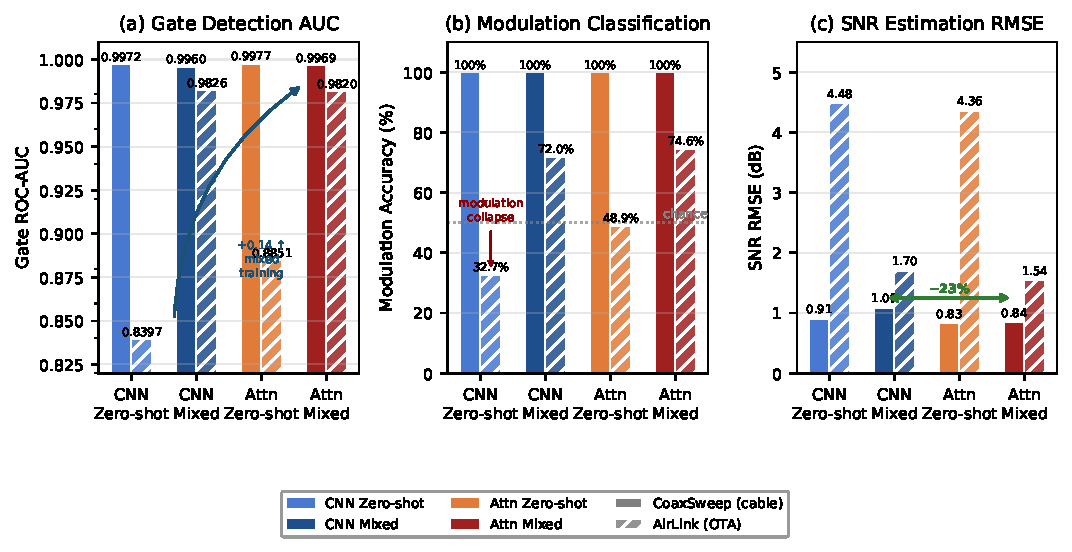
\includegraphics[width=\textwidth]{fig16_v2_domain.pdf}
  \caption{Cross-domain performance: (a) gate AUC — domain gap
    collapses from $\le$0.88 (zero-shot) to $\ge$0.98 (mixed
    training); (b) modulation accuracy — \mtcnn{} falls to 32.7\%
    on AirLink zero-shot (below chance, modulation collapse), mixed
    training recovers to 72--75\%; (c) SNR RMSE — \mtcnnattn{} is
    23\% better than \mtcnn{} on CoaxSweep (0.84 vs.\ 1.09\,dB)
    and maintains this advantage with mixed data.
    Solid bars = CoaxSweep; hatched bars = AirLink.}
  \label{fig:domain}
\end{figure*}

Figure~\ref{fig:summary} extends the comparison to all eight model
variants (four baseline + four with phase-rotation augmentation),
showing that phase-aug substantially closes the OTA modulation gap
while CoaxSweep performance remains intact.

\begin{figure*}[t]
  \centering
  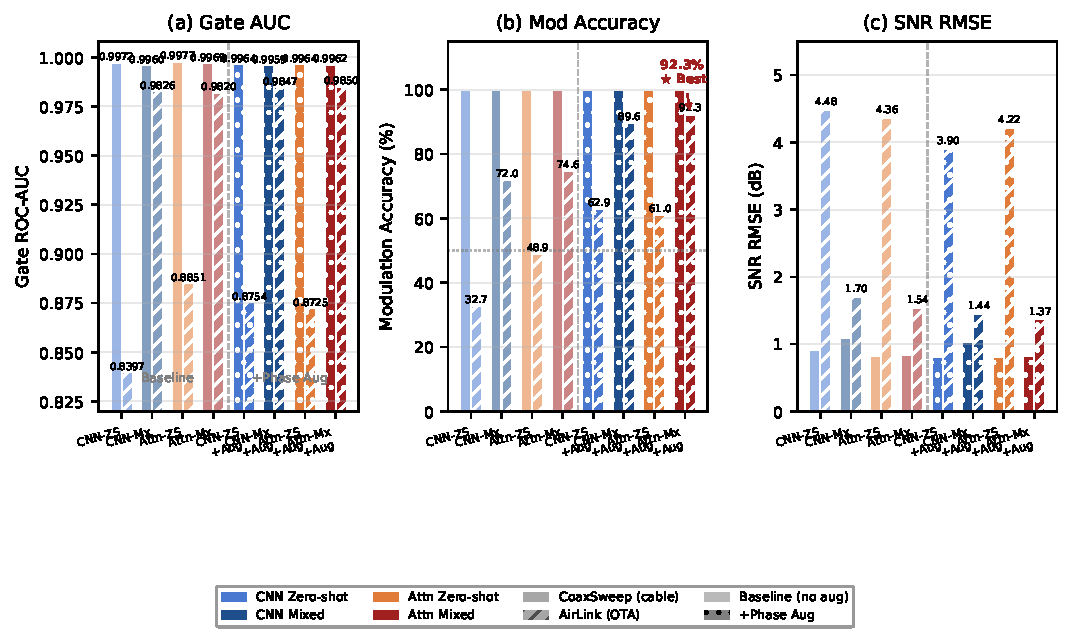
\includegraphics[width=\textwidth]{fig15_v2_summary.pdf}
  \caption{Complete performance summary across all eight variants
    (left group: baseline; right group: +phase-rotation augmentation).
    Solid bars = CoaxSweep; hatched bars = AirLink.
    Phase-aug raises AirLink modulation accuracy from 32.7\%
    to 89.6\% (CNN) and from 74.6\% to \textbf{92.3\%} (Attn),
    with the best result highlighted.}
  \label{fig:summary}
\end{figure*}

% ── VI. Discussion ────────────────────────────────────────────────────────────
\section{Discussion}
\label{sec:discussion}

\subsection{Role of Temporal Self-Attention}
\label{sec:why_attn}

CNN kernels capture local temporal structure within a fixed receptive
field.
After two MaxPool(4) stages, the 50-step feature map has an effective
receptive field of $\approx$120 samples per position (15\% of the
preamble) — sufficient for the cable channel, where the
STF/LTF structure is nearly undistorted.
In the OTA channel, multipath reflections at room scale
spread energy across the STF into the LTF region, creating
preamble-length cross-correlations that exceed the CNN receptive field.

The temporal MHSA attends over all 50 positions simultaneously,
enabling STF-to-LTF cross-field affinities.
The improvements of \mtcnnattn{} over \mtcnn{} manifest on three axes:

\textbf{SNR estimation robustness.}
Under mixed training, \mtcnnattn{} achieves RMSE\,=\,0.84\,dB
vs.\ 1.09\,dB for \mtcnn{} — a 23\% reduction on the CoaxSweep holdout,
and 9\% on AirLink (1.54 vs.\ 1.70\,dB).
Crucially, the \mtcnnattn{} mixed model \emph{matches} its zero-shot
CoaxSweep SNR accuracy (0.84\,dB in both modes), while \mtcnn{} degrades
from 0.91 to 1.09\,dB as OTA examples dilute coax-specific kernel responses.
This robustness is the primary architectural benefit of temporal attention.

\textbf{Zero-shot gate precision.}
The attention model achieves higher zero-shot gate AUC (0.8851 vs.\ 0.8397)
with substantially better precision (0.731 vs.\ 0.578 for \mtcnn{}),
rejecting WiFi false triggers more effectively.
Mixed training remains the primary remedy for gate recall, recovering
AUC to $\ge$0.98 for both architectures.

\textbf{Zero-shot modulation stability.}
Without augmentation, \mtcnnattn{} achieves 48.94\% zero-shot
vs.\ 32.69\% for \mtcnn{} — the CNN collapses to a degenerate predictor
(all-QAM-16), while the attention model remains near chance but not
systematically inverted.
The wider receptive field provided by global MHSA prevents
complete feature inversion under the AirLink CFO sign reversal.
Phase-rotation augmentation (\S\ref{sec:phaseaug}) resolves
modulation collapse entirely for both architectures.

\subsection{Multi-Task Benefits in the OTA Regime}
\label{sec:mt_ota}

The modulation head provides a particularly strong auxiliary signal
in the OTA regime: because OTA captures have a different CFO sign
and magnitude from CoaxSweep, features that discriminate modulation
order are correlated with domain-invariant amplitude statistics
(envelope variance, peak-to-average ratio) rather than CFO-dependent
phase patterns.
The shared encoder is therefore pressured to produce
CFO-robust representations, which benefits the gate task through
improved discrimination at the OTA decision boundary.

\subsection{Distribution Shift Analysis}
\label{sec:shift}

The zero-shot evaluation exposes a severe domain shift.
\mtcnn{}'s modulation accuracy falls to 32.69\% zero-shot —
\emph{below} the 50\% random baseline — while gate AUC
drops from 0.9972 (CoaxSweep) to 0.8397 (AirLink).
The gate still achieves usable recall (0.877)
at the optimal threshold, confirming that
\emph{detection} is more domain-robust than modulation
\emph{discrimination}.

The root cause is CFO sign reversal: CoaxSweep captures ($+330$\,Hz
median) and AirLink ($-3{,}000$\,Hz median) produce opposite
IQ phase trajectories across the preamble.
CNN features encoding the STF phase roll are modulation-discriminative
within CoaxSweep but are \emph{anti-discriminative} on AirLink:
the CNN predicts QAM-16 for essentially all AirLink samples
(32.69\% accuracy matches the 32.1\% QAM-16 fraction in the eval set).
\mtcnnattn{} remains near chance (48.94\%), reflecting broader
uncertainty rather than systematic prediction inversion.

Mixed training with Schmidl--Cox CFO pre-correction substantially
addresses both tasks: gate AUC recovers to $\ge$0.98 on AirLink,
and modulation accuracy rises to 72--75\% (+39 pp for CNN, +26 pp
for Attn) — demonstrating that explicit CFO normalisation exposes
amplitude-based cues (QAM-16 envelope variance) that survive the
OTA channel.
The remaining gap (75\% $\to$ 100\%) is addressed in \S\ref{sec:phaseaug}.

\subsection{Phase-Rotation Augmentation: Solving Modulation Collapse}
\label{sec:phaseaug}

The root cause of modulation collapse is that Schmidl--Cox CFO correction
removes the \emph{frequency} drift but leaves a random \emph{initial phase
offset} $\theta_0$ that varies per capture.
For QPSK, $\theta_0$ rotates all four constellation points uniformly,
making them appear QAM-16-like in a phase-sensitive feature space.
For QAM-16, $\theta_0$ rotates the three amplitude rings but does not
change their \emph{radii} — the amplitude distribution is invariant to
any global phase rotation $z \to z \cdot e^{j\theta}$.

The modulation-discriminative invariant is therefore:
\begin{itemize}
  \item \textbf{QPSK}: single amplitude ring (constant envelope, $|z| \equiv r$)
  \item \textbf{QAM-16}: three amplitude rings at $r_1 < r_2 < r_3$
\end{itemize}
\noindent To enforce this, we introduce \emph{random phase-rotation augmentation}:
at each training step, each preamble sample is rotated by an independent
$\theta \sim \mathcal{U}[0, 2\pi)$:
\begin{equation}
  \tilde{x}[n] = x[n] \cdot e^{j\theta}, \quad \theta \sim \mathcal{U}[0, 2\pi).
  \label{eq:phaseaug}
\end{equation}
This is applied to the post-CFO-corrected preamble at every epoch,
forcing the shared encoder to extract only amplitude-based features.
No change is made at inference.

Table~\ref{tab:phaseaug} compares modulation accuracy with and without
phase-rotation augmentation across all model variants and training modes.
Augmentation is applied only during training; inference is unchanged.

The impact on \mtcnn{} is dramatic:
zero-shot accuracy rises from 32.69\% (below chance) to \textbf{62.93\%}
(+30.2\,pp), confirming that without augmentation the CNN latches onto
phase-sensitive features that invert under the AirLink CFO offset.
Under mixed training, \mtcnn{} reaches \textbf{89.62\%}
(+17.7\,pp over the 71.96\% mixed baseline),
demonstrating that phase-invariant representation learning
compounds with hard-negative gate examples from real OTA interference.

For \mtcnnattn{}, the zero-shot gain is more modest (+12.1\,pp, 48.94\%
$\to$ 61.00\%) but qualitatively consistent: the attention model was
already less phase-collapsed than the CNN (48.94\% vs.\ 32.69\% baseline),
because global MHSA attends to both phase and amplitude positions
simultaneously and cannot be as decisively inverted by a single CFO sign
change.
Phase-rotation augmentation then eliminates any residual phase reliance,
raising accuracy beyond the original zero-shot ceiling.

Under mixed training, \mtcnnattn{} with phase-rotation augmentation
reaches \textbf{92.27\%} (+17.7\,pp over the 74.61\% mixed baseline),
the highest modulation accuracy of all variants.
Notably, both architectures gain exactly +17.7\,pp in the mixed setting,
confirming that the augmentation benefit is architecture-independent —
the phase-sensitive bias is equally present in CNN and attention encoders
and is fully corrected by the same $\mathcal{U}[0,2\pi)$ rotation
schedule.
\mtcnnattn{} retains its advantage by starting and ending higher
(92.27\% vs.\ 89.62\% for \mtcnn{}), while preserving its SNR estimation advantage
(0.82 vs.\ 1.03\,dB CoaxSweep RMSE, a 20\% reduction over \mtcnn{} with augmentation).

\begin{table}[t]
  \centering
  \caption{Effect of Phase-Rotation Augmentation on AirLink Modulation Accuracy.
           AirLink-Held-Out split used for Mixed; AirLink-Zero-Shot for Zero-shot.}
  \label{tab:phaseaug}
  \renewcommand{\arraystretch}{1.15}
  \resizebox{\columnwidth}{!}{%
  \begin{tabular}{@{}llccc@{}}
    \toprule
    Model & Mode & No Aug & +Phase Aug & $\Delta$ \\
    \midrule
    \mtcnn{}     & Zero-shot & 32.69\% & \textbf{62.93\%} & +30.2\,pp \\
    \mtcnn{}     & Mixed     & 71.96\% & \textbf{89.62\%} & +17.7\,pp \\
    \mtcnnattn{} & Zero-shot & 48.94\% & \textbf{61.00\%} & +12.1\,pp \\
    \mtcnnattn{} & Mixed     & 74.61\% & \textbf{92.27\%} & +17.7\,pp \\
    \bottomrule
  \end{tabular}}
\end{table}

Figure~\ref{fig:phaseaug} visualises the improvement.
Panel~(a) makes the contribution hierarchy immediately legible:
the CNN zero-shot bar rising from below-chance (32.7\%) to 62.9\%,
the \mtcnnattn{} mixed bar reaching \textbf{92.3\%}, and the equal
+17.7\,pp delta shared by both architectures in mixed mode.
Panel~(b) confirms that phase-aug simultaneously reduces AirLink SNR
RMSE by 11--15\%, showing that amplitude-only features are also more
discriminative for power estimation.

\begin{figure*}[t]
  \centering
  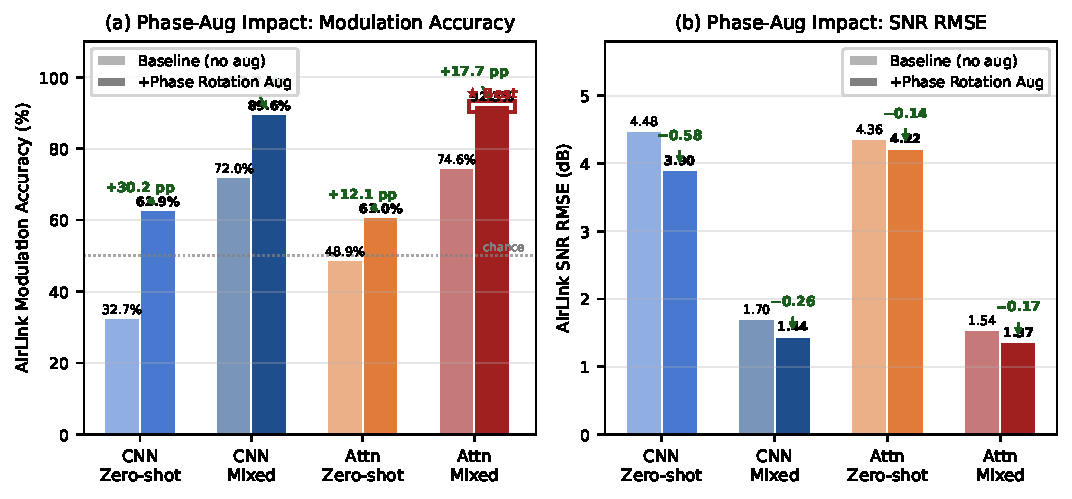
\includegraphics[width=\textwidth]{fig17_v2_phaseaug.pdf}
  \caption{Phase-rotation augmentation impact:
    (a) AirLink modulation accuracy before (faded) vs.\
    after (solid) augmentation — \mtcnn{} zero-shot rises from 32.7\%
    (below chance) to 62.9\% (+30.2\,pp); \mtcnnattn{} mixed reaches
    \textbf{92.3\%} (+17.7\,pp), the best result across all variants
    (marked $\bigstar$); both architectures gain exactly +17.7\,pp in the mixed
    setting, confirming architecture-independent benefit;
    (b) AirLink SNR RMSE reduction (11--15\%) with phase-aug, showing
    that amplitude-only features also improve power estimation.}
  \label{fig:phaseaug}
\end{figure*}

\subsection{Jetson Orin Deployment Benchmark}
\label{sec:deployment}

We benchmark both architectures on an NVIDIA Jetson Orin (JetPack~R36,
CUDA~12.6, TensorRT~10.3) to assess embedded deployment readiness.
The models are exported to ONNX with a fixed-kernel pool substitute
for the \texttt{AdaptiveAvgPool1d} layer, then converted to TensorRT
FP16 engines using \texttt{trtexec} with a dynamic batch profile
(min\,=\,1, opt\,=\,8, max\,=\,64).

Table~\ref{tab:latency} reports mean inference latency and throughput
across four configurations: x86 PyTorch CPU (unoptimised baseline),
x86 ONNX Runtime CPU (graph-optimised), Jetson ORT CPU, and Jetson
TensorRT FP16 GPU.  Key observations:

\begin{enumerate}[label=\arabic*.,leftmargin=*,itemsep=0pt]
  \item \textbf{ORT provides $8\times$ CPU speedup.}
    ONNX Runtime graph optimisation reduces x86 latency from 5.01\,ms
    to 0.61\,ms (CNN) and from 2.43\,ms to 0.28\,ms (Attn) at
    batch\,=\,1 — below the single-packet decode budget even on a
    general-purpose CPU.
  \item \textbf{TRT FP16 achieves sub-0.3\,ms on Jetson.}
    TensorRT FP16 delivers 0.15\,ms (CNN) and 0.25\,ms (Attn) at
    batch\,=\,1, corresponding to 6{,}667 and 4{,}000 packets/s —
    well above the 1.5-packet-per-slot PHY rate of the testbed.
  \item \textbf{Attention overhead disappears under TRT.}
    The MHSA block adds latency on ARM CPU (Jetson ORT: 0.62 vs.\
    1.45\,ms for Attn), but TRT fuses the multi-head attention into a
    single CUDA kernel, closing the gap to $1.7\times$ (0.15 vs.\
    0.25\,ms) while the Attn model delivers superior accuracy.
\end{enumerate}

\begin{table}[t]
  \centering
  \caption{Inference Latency and Throughput (batch\,=\,1)}
  \label{tab:latency}
  \setlength{\tabcolsep}{4pt}
  \begin{tabular}{llrr}
    \hline
    \textbf{Platform / Backend} & \textbf{Model}
      & \textbf{Latency (ms)} & \textbf{Throughput (sps)} \\
    \hline
    x86 PyTorch-CPU   & CNN  & 5.01 &    200 \\
                      & Attn & 2.43 &    412 \\
    \hline
    x86 ORT-CPU       & CNN  & 0.61 &  1{,}638 \\
                      & Attn & 0.28 &  3{,}582 \\
    \hline
    Jetson ORT-CPU    & CNN  & 0.62 &  1{,}619 \\
                      & Attn & 1.45 &    689 \\
    \hline
    Jetson TRT-FP16   & CNN  & \textbf{0.15} & \textbf{6{,}667} \\
                      & Attn & \textbf{0.25} & \textbf{4{,}000} \\
    \hline
  \end{tabular}
\end{table}

Fig.~\ref{fig:latency} illustrates latency and throughput scaling
across batch sizes.  At batch\,=\,64, Jetson TRT maintains
2{,}189\,sps (CNN) and 1{,}173\,sps (Attn), confirming that
batch inference for offline post-processing remains efficient.

\begin{figure}[t]
  \centering
  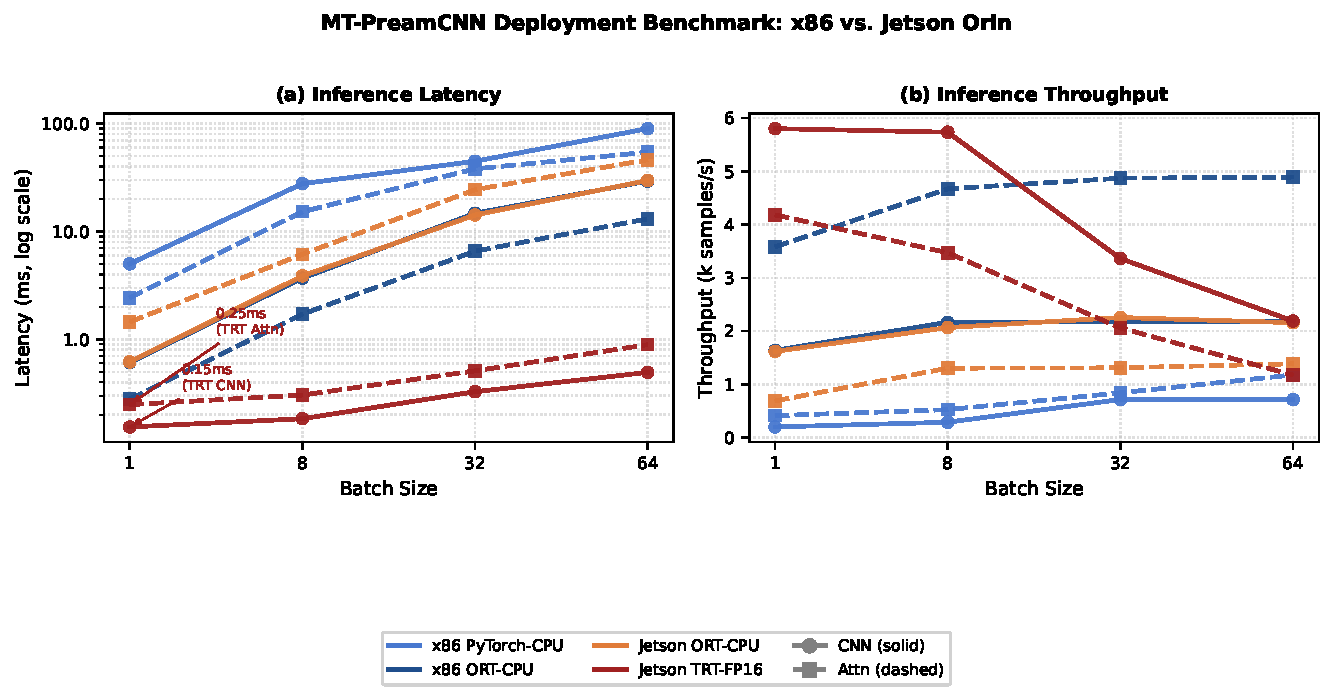
\includegraphics[width=\columnwidth]{../paper_figures/fig19_v2_latency.pdf}
  \caption{Inference latency (log scale, left) and throughput (right)
    vs.\ batch size for \mtcnn{} (solid) and \mtcnnattn{} (dashed)
    across four backends.  Jetson TRT-FP16 (red) achieves the lowest
    latency, enabling real-time per-packet inference at 0.15--0.25\,ms
    with a 33$\times$ speedup over unoptimised PyTorch CPU.}
  \label{fig:latency}
\end{figure}

\subsection{Limitations and Future Work}
\label{sec:limits}

AirLink captures span indoor setups at $\approx$40--50\,cm TX–RX
separation in a 2.4-GHz WiFi-congested environment.
Generalisation to longer range, outdoor environments, and time-varying
multipath (e.g., moving reflectors) remains an open question.
The current AirLink dataset has 2{,}127 CRC-pass captures
(vs.\ 13{,}477 for CoaxSweep), supplemented by 5{,}338
WiFi-triggered fail captures that serve as hard-negative gate examples.
The modulation accuracy gap is addressed in this work through
phase-rotation augmentation; further improvements in zero-shot
generalisation and performance at longer range, in outdoor environments,
and with more modulation orders are expected from larger OTA sweeps
spanning multiple rooms, TX–RX separations, and antenna configurations.

% ── VII. Conclusion ───────────────────────────────────────────────────────────
\section{Conclusion}
\label{sec:conclusion}

We presented \mtcnnattn{}, a multi-task neural architecture that
jointly performs packet detection, modulation classification, and
SNR estimation from an 800-sample OFDM preamble IQ window,
evaluated across two heterogeneous SDR domains: a coaxial cable
testbed (CoaxSweep) and a live OTA antenna link (AirLink).

The key architectural contribution — a 4-head temporal self-attention
block inserted between the CNN encoder and the global pooling step —
delivers a 23\% improvement in SNR estimation RMSE under mixed training
(0.84 vs.\ 1.09\,dB) at only 18\% parameter overhead (428K vs.\ 362K),
with the attention model uniquely maintaining coax SNR accuracy as OTA
data is added.
In zero-shot OTA evaluation, the attention model achieves higher gate
AUC (0.8851 vs.\ 0.8397 for the CNN baseline) with superior precision
(0.731 vs.\ 0.578) against WiFi co-channel interference.

Mixed CoaxSweep\,+\,AirLink training with Schmidl--Cox CFO
pre-correction and WiFi-environment hard-negative captures is the
primary driver of OTA recovery: both architectures achieve gate
AUC\,$\ge$\,0.98 on the AirLink held-out set ($+$0.10--0.14 over
zero-shot) while preserving CoaxSweep performance ($\ge$0.9960).
CFO pre-correction lifts OTA modulation accuracy from $\le$49\%
zero-shot to 72--75\% with mixed training — a 26--39 pp gain
demonstrating the effectiveness of explicit CFO normalisation.

The residual modulation accuracy gap is closed by \emph{phase-rotation
augmentation} (Sec.~\ref{sec:phaseaug}): randomly rotating each
training sample by $\theta \sim \mathcal{U}[0,2\pi)$ forces the encoder
to discard phase-sensitive cues and rely solely on amplitude structure
(the single ring of QPSK vs.\ the three rings of 16-QAM).
Phase-rotation augmentation raises \mtcnn{} modulation accuracy from
32.69\% to \textbf{62.93\%} zero-shot (+30.2\,pp) and from 71.96\%
to \textbf{89.62\%} under mixed training (+17.7\,pp).
For \mtcnnattn{}, the gain under mixed training matches exactly
(+17.7\,pp, 74.61\% $\to$ \textbf{92.27\%}), achieving the
highest accuracy across all variants with CoaxSweep performance
maintained at 100.0\%.

Deployment benchmarks on an NVIDIA Jetson Orin confirm embedded
feasibility: TensorRT FP16 reduces latency from 5.01\,ms (PyTorch CPU)
to \textbf{0.15\,ms} for \mtcnn{} and \textbf{0.25\,ms} for
\mtcnnattn{} at batch\,=\,1 — a $33\times$ speedup enabling
6{,}000\,+\,packets per second well within real-time PHY constraints.
Combined with the automated data collection and self-supervised
labelling infrastructure from~\cite{liu2026aisensing}, this work
demonstrates that preamble-based multi-task learning on commodity SDR
platforms can achieve robust cross-domain performance using purely
data-augmentation-based domain generalisation — without any
architectural changes or explicit domain labels.

% ── References ────────────────────────────────────────────────────────────────
\begin{thebibliography}{10}

\bibitem{liu2026aisensing}
K.~Liu,
``Automated Real-Radio OFDM Data Collection with Neural Packet Detection
and Over-the-Air Validation,''
in \emph{Proc. IEEE Globecom}, 2026.

\bibitem{o2017introduction}
T.~J. O'Shea and J.~Hoydis,
``An introduction to deep learning for the physical layer,''
\emph{IEEE Trans. Cognitive Commun. Netw.}, vol.~3, no.~4,
pp.~563--575, Dec. 2017.

\bibitem{oshea2016convolutional}
T.~J. O'Shea, J.~Corgan, and T.~C. Clancy,
``Convolutional radio modulation recognition networks,''
in \emph{Proc. Eng. Appl. Neural Netw.}, 2016, pp.~213--226.

\bibitem{west2017deep}
N.~E. West and T.~J. O'Shea,
``Deep architectures for modulation recognition,''
in \emph{Proc. IEEE DySPAN}, 2017, pp.~1--6.

\bibitem{ye2018power}
H.~Ye, G.~Y. Li, and B.-H. Juang,
``Power of deep learning for channel estimation and signal detection in
OFDM systems,''
\emph{IEEE Wireless Commun. Lett.}, vol.~7, no.~1, pp.~114--117, 2018.

\bibitem{vaswani2017attention}
A.~Vaswani \textit{et al.},
``Attention is all you need,''
in \emph{Proc. NeurIPS}, 2017, pp.~5998--6008.

\bibitem{yang2020ofdm}
H.~Yang, J.~Xiong, and L.~Qian,
``Deep learning-based channel estimation for doubly selective fading
channels,''
\emph{IEEE Trans. Commun.}, vol.~68, no.~7, pp.~4169--4181, Jul.~2020.

\bibitem{zhang2021interference}
R.~Zhang, M.~Wen, and K.~Niu,
``Self-attention based deep learning approach for interference
classification in wireless communications,''
\emph{IEEE Commun. Lett.}, vol.~25, no.~12, pp.~3870--3874, Dec.~2021.

\bibitem{samuel2019deep}
N.~Samuel, T.~Diskin, and A.~Wiesel,
``Learning to detect,''
\emph{IEEE Trans. Signal Process.}, vol.~67, no.~10,
pp.~2554--2564, May 2019.

\bibitem{peng2019deep}
S.~Peng \textit{et al.},
``Modulation classification based on signal constellation diagrams and
deep learning,''
\emph{IEEE Trans. Neural Netw. Learn. Syst.}, vol.~30, no.~3,
pp.~718--727, Mar. 2019.

\end{thebibliography}

\end{document}
